\chapter{DESAIN DAN PERANCANGAN}
    Pada bab ini dibahas mengenai analisis dan perancangan sistem.
    
    \section{Deskrisi Umum Sistem}
    	Sistem yang akan dibuat dalam tugas akhir ini adalah sistem yang digunakan untuk melacak perubahan konfigurasi perangkat jaringan. Sistem terhubung dengan perangkat jaringan dan menyimpan semua versi perubahan dari file konfigurasi perangkat jaringan. Sistem bisa mengatur versi konfigurasi yang dibutuhkan oleh perangkat jaringan untuk dipasang pada perangkat jaringan.\\
    	
    	\indent Sistem memiliki server repositori untuk menyimpan file konfigurasi dari perangkat jaringan yang dikirim melalui protokol TFTP dan FTP menyesuaikan protokol yang didukung oleh perangkat jaringan. Di dalam sistem terdapat \textit{Repository Observer} yang berfungsi untuk melihat perubahan di dalam repositori. Ketika ada perubahan, sistem otomatis melakukan commit terhadap Git untuk mencatat perubahan dari file.\\
    	
    	\indent Di dalam sistem terdapat dua \textit{web service} yang digunakan yaitu Gitea dan Flask. Web service tersebut digunakan untuk menerjemahkan instruksi dari administrator kepada sistem sesuai dengan diagram penggunaan pada Gambar \ref{usecase}. 
	
    \section{Kasus Penggunaan}
    	Dalam sistem ini hanya ada satu aktor yaitu \textit{administrator} jaringan yang akan mengatur penyimpanan konfigurasi. Diagram kasus penggunaan digambarkan pada Gambar \ref{usecase}.
        \begin{figure}[H]
			\centering
			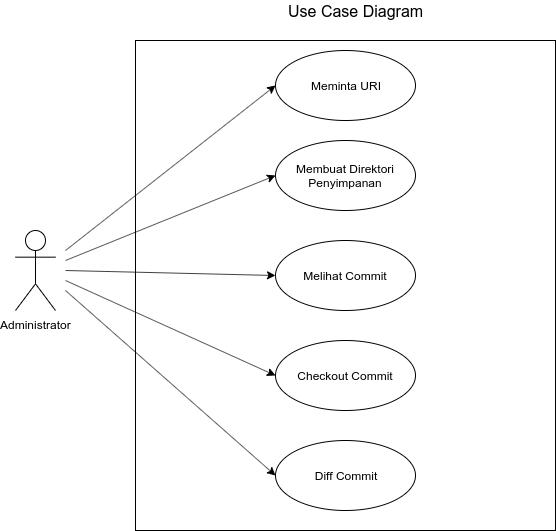
\includegraphics[width=8cm,height=8cm]{Images/C-3/UC.png}
			\caption{Diagram Kasus Penggunaan}
			\label{usecase}
		\end{figure}
        \indent Diagram kasus penggunaan pada Gambar \ref{usecase} dideskripsikan masing-masing pada Tabel \ref {tabelKodeKasusPenggunaan}.
        
        \begin{longtable}{|p{0.25\textwidth}|p{0.24\textwidth}|p{0.35\textwidth}|} % L = Rata kiri untuk setiap kolom, | = garis batas vertikal.
		    	
		    	% Kepala tabel, berulang di setiap halaman
		    
		    	
		    	 \caption{Daftar Kode Kasus Penggunaan} \label{tabelKodeKasusPenggunaan} \\
		    	\hline
		    		\textbf{Kode Kasus Penggunaan} & \textbf{Nama Kasus Penggunaan} & \textbf{Keterangan} \\ \hline
		    	\endfirsthead
		    	\caption[]{Daftar Kode Kasus Penggunaan}   \\
		    	\hline
		    		\textbf{Kode Kasus Penggunaan} & \textbf{Nama Kasus Penggunaan} & \textbf{Keterangan} \\ \hline
		    	\endhead
		    	\endfoot
		    	\endlastfoot
		    	
		    	UC-0001 & Meminta URI. & \textit{Administrator} dapat meminta alamat URI untuk mengirim konfigurasi dari perangkat jaringan.\\ \hline
		    	UC-0002 & Membuat Direktori Penyimpanan.  & \textit{Administrator} dapat membuat direktori untuk menyimpan konfigurasi dari perangkat jaringan.\\ \hline
		    	UC-0003 & Melihat Commit. & \textit{Administrator} dapat melihat riwayat commit dalam repositori perangkat. \\ \hline
		    	UC-0004 & Checkout Commit. & Administrator dapat berpindah commit (checkout) sesuai dengan versi commit yang diinginkan. \\ \hline
				UC-0005 & Diff Commit. & Administrator dapat melihat perbedaan antara commit satu dengan lainnya. \\ \hline		    	
		    \end{longtable}

	\section{Arsitektur Sistem}
		Pada sub-bab ini, dibahas mengenai tahap analisis dan kebutuhan bisnis dan desain dari sistem yang akan dibangun. Arsitektur sistem secara umum ditunjukkan pada Gambar \ref{DesainUmumSistem}.\\
		\begin{figure}[H]
			\centering
			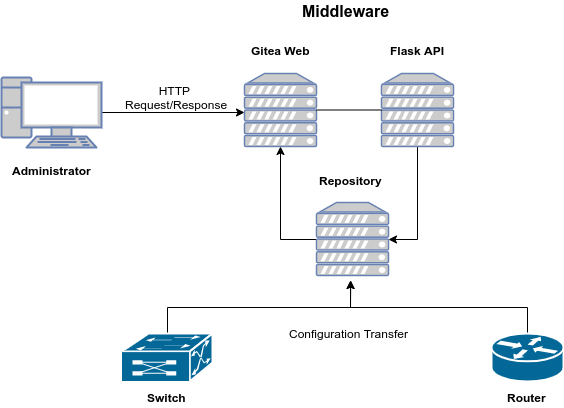
\includegraphics[width=\textwidth]{Images/C-3/Desain-Umum-TA-2.png}
			\caption{Desain Umum Sistem}
			\label{DesainUmumSistem}
		\end{figure}

		\subsection{Desain Umum Sistem}
			Berdasarkan yang dijelaskan pada deskripsi umum sistem, dapat diperoleh kebutuhan sistem sebagai berikut:
			\begin{enumerate}
				\item \textit{Repository Server} untuk menyimpan file konfigurasi dari perangkat jaringan.
				\item \textit{Repository Observer} untuk melihat perubahan file yang disimpan di dalam repository server.
				\item \textit{Web Service} untuk menerjemahkan intruksi dari admin kepada sistem.
			\end{enumerate}
                
                
		\subsection{Perancangan Repositori Perangkat }
			\begin{figure}[H]
				\centering
				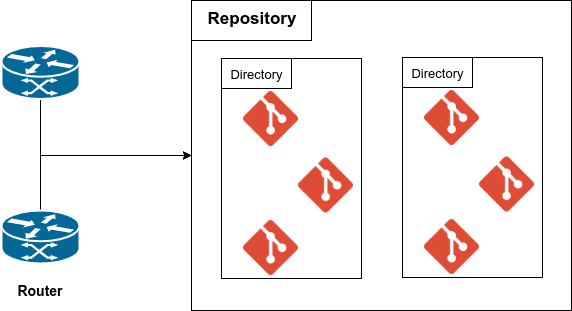
\includegraphics[width=\textwidth]{Images/C-3/Repository.png}
				\caption{Desain Repositori Perangkat}
				\label{DesainRepositoriPerangkat}
			\end{figure}
			Repositori perangkat adalah komponen untuk menyimpan file konfigurasi perangkat jaringan. Repositori perangkat merupakan direktori yang menjadi tujuan pegiriman file konfigurasi perangkat jaringan. Pengiriman file konfigurasi menggunakan TFTP dan FTP. Di dalam repositori perangkat, direktori akan dibedakan berdasarkan protokol pengiriman dan nama perangkat. Setiap perangkat memiliki direktori masing-masing dan setiap direktori merupakan \textit{Git Repository}.\\ 

		
            
        \subsection{Perancangan \textit{Repository Observer}}
            Pada sistem ini Middleware harus bisa mengamati repositori perangkat jaringan secara berkelanjutan dan melakukan update pada history commit pada repositori. Untuk melakukan hal tersebut modul watchdog di dalam middleware yang akan melihat setiap perubahan pada respositori perangkat jaringan. Modul watchdog berjalan sebagai thread yang menunggu perubahan kondisi di dalam repositori. Ketika thread mengidentifikasi ada perubahan di dalam repositori maka thread akan menjalankan perintah commit menggunakan modul gitPython yang terintegrasi dengan middleware.
            \begin{figure}[H]
            	\centering
            	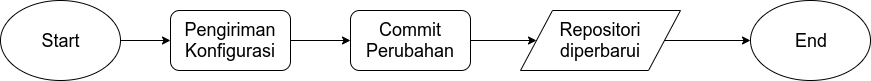
\includegraphics[width=10cm,height=1cm]{Images/C-3/AlurPengirimanFile.png}
            	\caption{Alur Pengiriman File}
            	\label{desain:pengiriman file}
            \end{figure}
	        \indent Repository Observer juga mengatur pembentukan cabang dari repositori penyimpanan konfigurasi perangkat jaringan. Alur pembuatan cabang dari repositori seperti pada gambar \ref{CreateBranch}.
	        \begin{figure}[H]
	        	\centering
	        	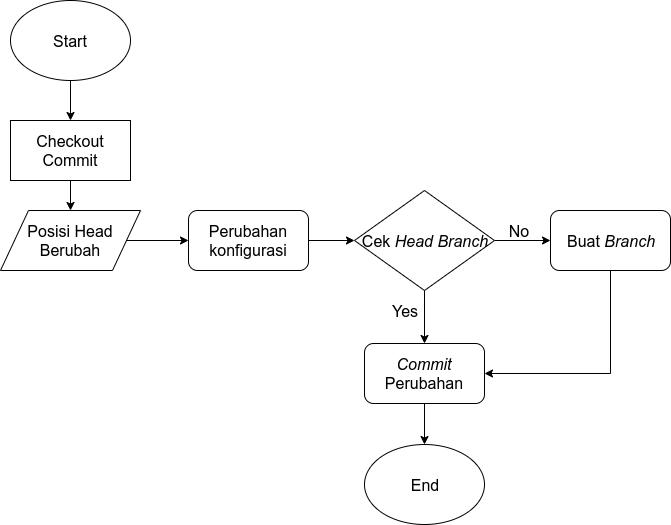
\includegraphics[width=\textwidth]{Images/C-3/CreateBranch.png}
	        	\caption{Alur Pembuatan Branch}
	        	\label{CreateBranch}
	        \end{figure}
        
        
        \subsection{Perancangan Web \textit{Service}}
        	Dalam sistem yang dibangun, web service digunakan untuk menerjemahkan permintaan dari adiministrator jaringan. Web service memiliki antarmuka dan rute dengan parameter nama repositori dan permintaan fitur yang diinginkan. Setiap rute akan diproses oleh \textit{Middleware} dan kemudian mengirimkan respon kepada administrator.\\
        	\indent Terdapat dua web service yang digunakan dalam sistem pelacakan konfigurasi perangkat jaringan yakni Gitea webapp dan flask API. Gitea webapp digunakan untuk menampilkan user interface dari sistem sedangkan flask API digunakan untuk melakukan operasi pada repositori lokal berdasarkan permintaan dari gitea webapp. 
         	\begin{figure}[H]
         		\centering
         		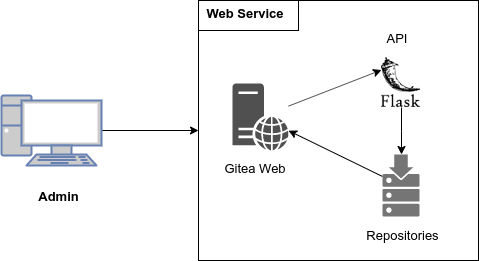
\includegraphics[width=\textwidth]{Images/C-3/Web_Service.png}
         		\caption{Perancangan Web \textit{Service}}
         		\label{WebService}
         	\end{figure}
        
       
            
        